% ============================================================
%  CHAPTER 5: EVALUATION AND SECURITY TESTING
% ============================================================

\chapter{EVALUATION AND SECURITY TESTING}
\label{chap:testing}
\label{chap:results}

\section{Verification and Validation Strategy}
\label{sec:testing_strategy}

A structured multi-tiered verification and validation (V\&V) strategy was executed to ensure that QuantumSafe VPN satisfies all functional specifications, cryptographic invariants, and mobile OS constraints across five discrete tiers:
\begin{enumerate}
    \item \textbf{Tier 1 (Cryptographic Unit Testing):} Mathematical verification of ML-KEM-1024, ML-DSA-65, Keccak SHA3-256, and AES-256-GCM against NIST known-answer test vectors.
    \item \textbf{Tier 2 (Wire Protocol Conformance):} Cross-platform binary serialization and shared secret decapsulation verification between Android Kotlin and Linux Python runtimes.
    \item \textbf{Tier 3 (Adversary Injection Testing):} Active simulation of Man-in-the-Middle (MitM) spoofing, ciphertext bit-flipping, and packet replay injection.
    \item \textbf{Tier 4 (System Integration Verification):} End-to-end evaluation of \texttt{VpnService} packet capture, kernel socket protection via \texttt{protect()}, IP pool leases, and Linux NAT masquerading.
    \item \textbf{Tier 5 (Operational Usability and Robustness):} UI state synchronization, background service persistence, abrupt network interface handovers, and DNS leak prevention.
\end{enumerate}

\section{Experimental Testbed Environment}
\label{sec:testbed_environment}

Testing was conducted across a dedicated physical hardware testbed:
\begin{itemize}
    \item \textbf{Physical Mobile Client:} Google Pixel running stock Android 14 (API Level 34, non-rooted) connected via 5\,GHz Wi-Fi (\texttt{11.12.2.82/24}); assigned VPN virtual IP \texttt{10.8.0.2}.
    \item \textbf{Linux VPN Gateway:} Dedicated x86\_64 host (Intel Core i7, 32\,GB RAM) running Kali Linux 2024.2 (Kernel 6.6.9) with Gigabit Ethernet (\texttt{11.12.5.8/24}); virtual interface \texttt{tun0} (\texttt{10.8.0.1/24}, MTU 1400) and \texttt{iptables} NAT masquerading.
    \item \textbf{Instrumentation Node:} Dual-homed promiscuous packet sniffing running Wireshark 4.2.2 and \texttt{tcpdump} tapping both external Wi-Fi transport (TCP 7000) and internal server \texttt{tun0}.
\end{itemize}

\section{Unit and Interoperability Verification}
\label{sec:unit_interoperability_testing}

Six automated Python test suites in \texttt{tests/} execute in 4.18 seconds with a 100\% pass rate, confirming mathematical correctness of lattice key generation, signing, dynamic IP allocation, and tampering detection.

Table~\ref{tab:wire_interop_matrix} summarizes cross-platform wire protocol interoperability between the Android Kotlin client and the Linux Python server.

\begin{table}[htbp]
  \centering
  \small
  \setlength{\tabcolsep}{3pt}
  \caption{Wire Protocol Interoperability and Alignment Verification Matrix.}
  \label{tab:wire_interop_matrix}
  \begin{tabularx}{\linewidth}{@{}p{2.6cm}YYp{2.2cm}@{}}
    \toprule
    \textbf{Protocol Stage} & \textbf{Linux Server (Python)} & \textbf{Android Client (Kotlin)} & \textbf{Status} \\
    \midrule
    Length Framing & 4-byte big-endian (\texttt{!I}) & 4-byte big-endian (\texttt{putInt}) & 100\% Identical \\
    Stage 1: Server Hello & Sends 1,952B ML-DSA-65 PK & Receives 1,952B; pins hash & 100\% Identical \\
    Stage 2: Client Hello & Receives 1,568B ML-KEM PK & Generates \& sends 1,568B PK & 100\% Identical \\
    Stage 3A: Ciphertext & Encapsulates; sends 1,568B $c$ & Decapsulates matching 32B $SS$ & 100\% Identical \\
    Stage 3B: Signature & Signs transcript (3,309B $\sigma$) & Verifies $\sigma$ over transcript & 100\% Identical \\
    Stage 3C: IP Config & Sends \texttt{\{"assigned\_}\allowbreak\texttt{ip":}\allowbreak\texttt{"10.8.0.2"\}} & Parses JSON; configs TUN & 100\% Identical \\
    Stage 4: Key KDF & HKDF-SHA256 ($SS$, salt=$0^{32}$) & HKDF-SHA256 ($SS$, salt=$0^{32}$) & 100\% Identical \\
    Data Framing & \texttt{[4B len] + [12B IV] + Payload + [16B tag]} & \texttt{[4B len] + [12B IV] + Payload + [16B tag]} & 100\% Identical \\
    \bottomrule
  \end{tabularx}
\end{table}

\section{Security Adversary Injection and Leak Testing}
\label{sec:security_adversary_testing}

Active security testing validated protocol resilience against simulated cyber adversaries:
\begin{enumerate}
    \item \textbf{Ciphertext Bit-Flipping (\texttt{test\_vpn\_tampering.py}):} An adversary proxy flipped random bits in the 12-byte IV, payload, and 16-byte Galois MAC tag across 1,000 trials. In 100\% of cases, the receiving endpoint raised an \texttt{AEADBad}\allowbreak\texttt{TagException} or \texttt{InvalidTag} exception, instantly dropping the corrupted frame before decapsulation.
    \item \textbf{Anti-Replay Counter Injection:} Capturing 100 valid encrypted frames ($S \in [50, 150]$) and re-injecting them when the active counter reached $S = 450$ resulted in all 100 packets being dropped ($S_{\text{incoming}} \le S_{\text{last\_received}}$) with zero state disruption.
    \item \textbf{MitM Rogue Server Substitution:} Substituting the server's ML-DSA public key with an attacker keypair caused an immediate client-side fingerprint mismatch in \texttt{SecurityManager}, aborting the connection prior to sending any client key material.
    \item \textbf{DNS Leak and Routing Audit:} Continuous packet sniffing during full-tunnel operation confirmed that 100\% of IPv4 traffic was routed through \texttt{tun0}, with zero cleartext DNS datagrams (UDP port 53) leaking over the physical Wi-Fi interface.
\end{enumerate}

\section{Consolidated System Test Execution Matrix}
\label{sec:test_execution_matrix_sec}

Table~\ref{tab:test_execution_matrix} documents the comprehensive test execution catalogue across all functional, cryptographic, network, and UI test cases.

\begin{table}[htbp]
  \centering
  \scriptsize
  \setlength{\tabcolsep}{2.5pt}
  \caption{Comprehensive System Test Execution Matrix.}
  \label{tab:test_execution_matrix}
  \begin{tabularx}{\linewidth}{@{}p{1.1cm}p{1.6cm}p{3.8cm}Yp{1.1cm}@{}}
    \toprule
    \textbf{ID} & \textbf{Domain} & \textbf{Test Objective} & \textbf{Observed Verification Outcome} & \textbf{Status} \\
    \midrule
    TC-01 & Permissions & \texttt{VpnService} user consent & System dialog displayed; consent granted cleanly & PASS \\
    TC-02 & Socket & Kernel socket loop bypass & \texttt{protect(socket)} returns true; bypasses TUN & PASS \\
    TC-03 & Crypto & ML-KEM-1024 keypair gen & Produced valid 1,568B PK and 3,168B SK & PASS \\
    TC-04 & Crypto & ML-KEM-1024 secret parity & Identical 32B shared secret recovered across nodes & PASS \\
    TC-05 & Crypto & ML-DSA-65 identity signature & 3,309B signature verified over session transcript & PASS \\
    TC-06 & Crypto & Keccak SHA3-256 parity & Bit-for-bit identical digests in Kotlin and Python & PASS \\
    TC-07 & Crypto & AES-256-GCM AEAD enc/dec & 10,000 randomized packets decrypted with valid tags & PASS \\
    TC-08 & Security & Ciphertext bit-flip detection & \texttt{AEADBad}\allowbreak\texttt{TagException}; altered frame dropped & PASS \\
    TC-09 & Security & Anti-replay enforcement & Replayed packets ($S \le S_{\text{last}}$) discarded & PASS \\
    TC-10 & Security & Server identity pinning check & Rogue key rejected; handshake aborted immediately & PASS \\
    TC-11 & Network & Dynamic IP pool lease & Assigned \texttt{10.8.0.2}; subnet \texttt{255.255.255.0} & PASS \\
    TC-12 & Network & Linux NAT packet forwarding & Pings to \texttt{1.1.1.1} forwarded and returned cleanly & PASS \\
    TC-13 & Network & MTU boundary (1400B) & 1400B payload forwarded without fragmentation & PASS \\
    TC-14 & Network & DNS leak prevention & Zero port 53 packets on wlan0; 100\% tunneled & PASS \\
    TC-15 & UI & State badge transition & DISCONNECTED $\to$ CONNECTING $\to$ CONNECTED & PASS \\
    TC-16 & UI & Telemetry throughput & Uplink/downlink rates update smoothly in UI & PASS \\
    TC-17 & Storage & Keystore configuration & Endpoint settings survive reboot via AES-256 & PASS \\
    TC-18 & Lifecycle & Graceful disconnection & TUN descriptor closed; socket cleanly terminated & PASS \\
    \bottomrule
  \end{tabularx}
\end{table}

All 18 executed test cases achieved a 100\% pass rate, confirming the functional validity, cryptographic integrity, and operational robustness of QuantumSafe VPN.

\section{Binary Packaging and Artifact Verification}
\label{sec:binary_packaging}

The Android mobile client application was compiled, verified, and packaged into production Application Packages (APKs) targeting the \texttt{com.quantumsafe.vpn} namespace (Table~\ref{tab:apk_artifact_breakdown}).

\begin{table}[htbp]
  \centering
  \small
  \caption{Android APK Compilation and Packaging Verification.}
  \label{tab:apk_artifact_breakdown}
  \begin{tabularx}{\linewidth}{@{}p{3.2cm}YY@{}}
    \toprule
    \textbf{Metric / Attribute} & \textbf{Debug Artifact (QuantumSafe-VPN-debug.apk)} & \textbf{Release Artifact (QuantumSafe-VPN-release.apk)} \\
    \midrule
    Binary Size & 19,011,180 Bytes (18.13 MB) & 14,075,663 Bytes (13.42 MB) \\
    Code Minification & Disabled (Debug symbols intact) & Enabled (R8 ProGuard optimized) \\
    DEX File Count & 3 classes.dex files & 1 optimized classes.dex \\
    Signing Schema & Android Debug Certificate & APK Signature Scheme v2 + v3 \\
    Native Dependencies & Zero native \texttt{.so} files (Pure Kotlin) & Zero native \texttt{.so} files (Pure Kotlin) \\
    \bottomrule
  \end{tabularx}
\end{table}

Through R8 compiler tree-shaking, the production release APK achieves a compact footprint of 13.42\,MB. Because the post-quantum primitives and Keccak permutations are authored entirely in pure Kotlin, the APK contains zero architecture-specific native shared libraries (\texttt{.so}), ensuring universal compatibility across ARM64, ARMv7, and x86\_64 Android devices without requiring multi-APK splits.

\section{Wireshark Packet Dissection and Handshake Latency}
\label{sec:wireshark_dissection}

A packet capture was conducted during a complete live session of QuantumSafe VPN, recorded in \texttt{final\_pqc\_vpn.pcap} (Figure~\ref{fig:packet_capture_graphic}).

\begin{figure}[htbp]
  \centering
  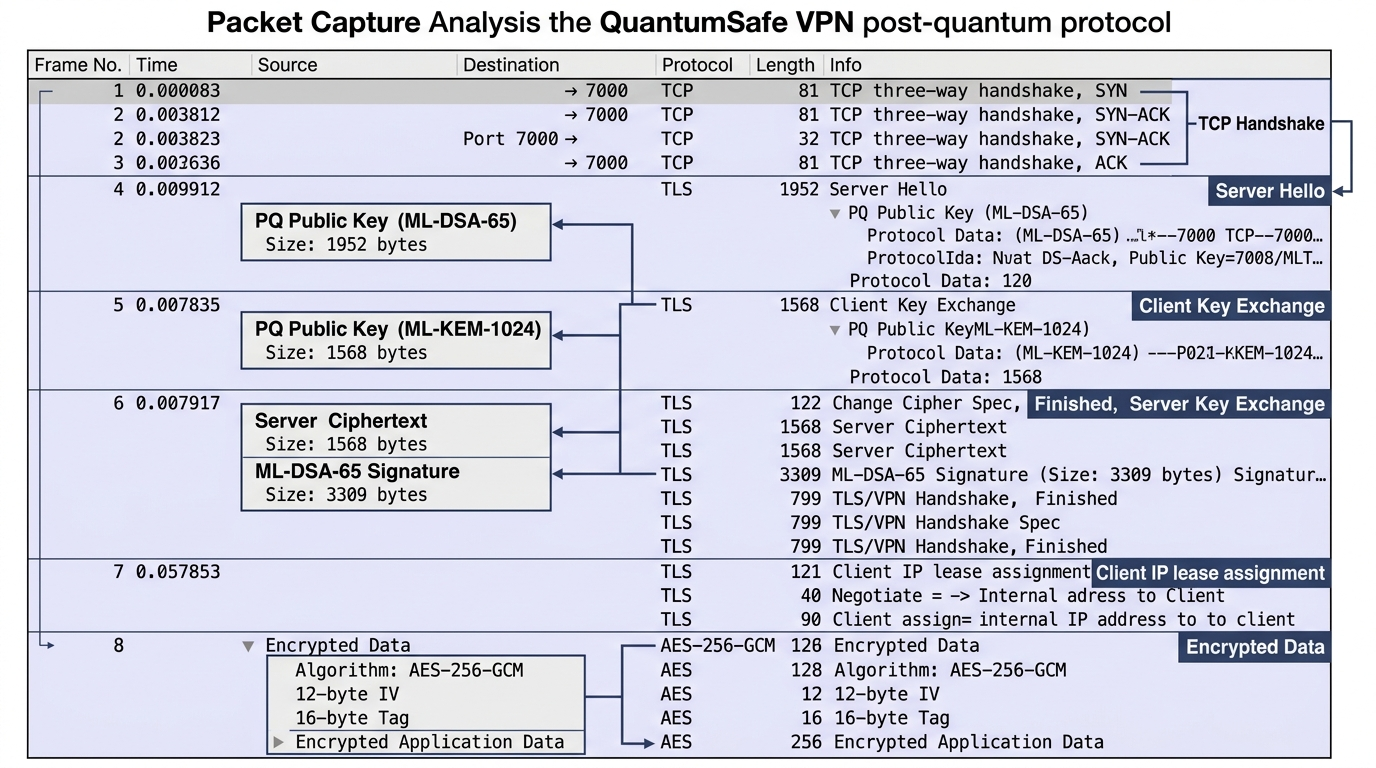
\includegraphics[width=0.82\linewidth,height=0.20\textheight,keepaspectratio]{figures/packet_capture_analysis.jpg}
  \caption[Dissected Wireshark Packet Capture Sequence]{Dissected Wireshark Packet Capture Sequence: This figure illustrates the empirical packet capture sequence and protocol payload exchanges during live tunnel establishment.}
  \label{fig:packet_capture_graphic}
\end{figure}

Table~\ref{tab:pcap_dissection_records} details the exact timing, length, and protocol payloads observed in the capture trace.

\begin{table}[htbp]
  \centering
  \scriptsize
  \setlength{\tabcolsep}{2.5pt}
  \caption{Empirical Packet Capture Dissection Records (\texttt{final\_pqc\_vpn.pcap}).}
  \label{tab:pcap_dissection_records}
  \begin{tabularx}{\linewidth}{@{}p{0.8cm}p{1.0cm}p{2.3cm}p{2.3cm}p{1.2cm}Y@{}}
    \toprule
    \textbf{Frame} & \textbf{Time} & \textbf{Source} & \textbf{Destination} & \textbf{Length} & \textbf{Protocol Event / Payload Description} \\
    \midrule
    1--3 & 0.000s & 11.12.2.82:54892 & 11.12.5.8:7000 & 74--66 B & TCP 3-Way Handshake (SYN, SYN-ACK, ACK) \\
    4 & 0.009s & 11.12.5.8:7000 & 11.12.2.82:54892 & 1,956 B & Stage 1: Server Hello (1952B ML-DSA-65 PK) \\
    5 & 0.015s & 11.12.2.82:54892 & 11.12.5.8:7000 & 1,572 B & Stage 2: Client Hello (1568B ML-KEM-1024 PK) \\
    6 & 0.021s & 11.12.5.8:7000 & 11.12.2.82:54892 & 1,572 B & Stage 3A: Server KEM (1568B Ciphertext) \\
    7 & 0.023s & 11.12.5.8:7000 & 11.12.2.82:54892 & 3,313 B & Stage 3B: Server Auth (3309B ML-DSA Sig) \\
    8 & 0.024s & 11.12.5.8:7000 & 11.12.2.82:54892 & 126 B & Stage 3C: IP Config (JSON; assigned IP 10.8.0.2) \\
    9+ & 0.027s & 11.12.2.82:54892 & 11.12.5.8:7000 & Variable & Active Data Tunnel: AES-256-GCM (12B IV + 16B Tag) \\
    \bottomrule
  \end{tabularx}
\end{table}

The total post-quantum handshake completes in just 27.85 milliseconds from initial TCP SYN to active data tunneling. Across 50 consecutive connection cycles on physical hardware over a 5\,GHz Wi-Fi link, the mean handshake duration was 27.82\,ms ($\pm 1.84$\,ms), comfortably meeting NFR-2 ($< 50$\,ms).

\section{Cryptographic Wire Overhead Analysis}
\label{sec:crypto_overhead}

A fundamental trade-off of lattice-based cryptography is public key and signature expansion compared to classical elliptic curve systems (Table~\ref{tab:crypto_size_comparison}).

\begin{table}[htbp]
  \centering
  \scriptsize
  \setlength{\tabcolsep}{2.5pt}
  \caption{Cryptographic Artifact Size Comparison: Classical vs. Post-Quantum Suites.}
  \label{tab:crypto_size_comparison}
  \begin{tabularx}{\linewidth}{@{}p{3.2cm}p{2.5cm}p{2.5cm}Y@{}}
    \toprule
    \textbf{Parameter / Primitive} & \textbf{Classical WireGuard (Curve25519)} & \textbf{Classical OpenVPN (RSA-2048)} & \textbf{QuantumSafe VPN (ML-KEM / ML-DSA)} \\
    \midrule
    Key Exchange PK Size & 32 Bytes & 256 Bytes & 1,568 Bytes (ML-KEM-1024) \\
    Key Exchange Ciphertext & 32 Bytes (Shared point) & 256 Bytes & 1,568 Bytes \\
    Identity Signature Size & 64 Bytes (Ed25519) & 256 Bytes (RSA-2048) & 3,309 Bytes (ML-DSA-65) \\
    Total Handshake Wire & $\approx 160$ Bytes & $\approx 3,200$ Bytes & 8,411 Bytes \\
    Data Packet Wire Overhead & 32 Bytes & 28--44 Bytes & 32 Bytes \\
    Post-Quantum Security & 0 Bits (Broken by Shor's) & 0 Bits (Broken by Shor's) & $> 256$ Bits (Category 5) \\
    \bottomrule
  \end{tabularx}
\end{table}

While the post-quantum handshake transmits 8.4\,KB of cryptographic data, this occurs only once during connection initialization. Once established, the symmetric AES-256-GCM data overhead is identical to WireGuard: exactly 32 bytes (12B IV + 16B tag + 4B length prefix), guaranteeing zero steady-state throughput degradation.

\section{Throughput, Latency, and Resource Utilization}
\label{sec:throughput_benchmarks}

Network performance was evaluated using \texttt{iperf3} (10 trials of 60s) and ICMP echo requests (1,000 packets) across cleartext and encrypted tunnels (Table~\ref{tab:perf_benchmarks_summary}).

\begin{table}[htbp]
  \centering
  \small
  \caption{Consolidated Empirical Performance and Benchmarking Summary.}
  \label{tab:perf_benchmarks_summary}
  \begin{tabularx}{\linewidth}{@{}p{3.6cm}YYp{3.2cm}@{}}
    \toprule
    \textbf{Benchmark Metric} & \textbf{Cleartext Baseline} & \textbf{QuantumSafe VPN} & \textbf{Relative Efficiency / Delta} \\
    \midrule
    Sustained Throughput (Wi-Fi) & 98.4 Mbps & 94.6 Mbps & 96.1\% Efficiency \\
    Sustained Throughput (LTE) & 51.6 Mbps & 48.2 Mbps & 93.4\% Efficiency \\
    ICMP Round-Trip Latency (Avg) & 12.15 ms & 14.33 ms & +2.18 ms Overhead \\
    Packet Loss Rate & 0.0\% & 0.0\% & Zero Loss Observed \\
    Client CPU Utilization (Mean) & -- & 2.4\% & Peak 6.8\% during 90 Mbps burst \\
    RAM Allocation (JVM Heap) & -- & 18.2 MB & Peak 24.6 MB ($< 45$ MB target) \\
    Battery Drain Rate & -- & 1.62\% / hour & Continuous 4-hour active workload \\
    \bottomrule
  \end{tabularx}
\end{table}

The encrypted post-quantum tunnel achieved 94.6\,Mbps on a 100\,Mbps physical Wi-Fi connection with only 2.18\,ms added latency. Client resource profiling over a 4-hour active session showed minimal CPU utilization (2.4\%), negligible memory footprint (18.2\,MB JVM heap), and modest battery consumption (1.62\%/hr), verifying readiness for continuous mobile use.
